%
% Transportation Research Board conference paper template
% version 1.1
% 
% David R. Pritchard, http://davidpritchard.org
%   1.0 - Mar. 2009
%   1.1 - Sep. 2011, fixes for captions
%   2.0 - Mar. 2012, Reorganized title page incl. automatic counters

% PAGE LAYOUT
%------------------------------------------

% Custom paper settings...
\documentclass[titlepage,oneside,12pt]{article}

\oddsidemargin 0.0in
\topmargin -0.5in
\headheight 0.3in
\headsep 0.2in
\textwidth 6.5in
\textheight 9.0in
\setlength{\parindent}{0.5in}

% PAGE HEADER
%------------------------------------------
% Adjust the header text below (INSERT AUTHORS HERE)
\oddsidemargin 0.0in
\usepackage[tiny,rm]{titlesec}
\newpagestyle{trbstyle}{
	\sethead{Guilliard}{}{\thepage}
}
\pagestyle{trbstyle}

% HEADINGS
%------------------------------------------
\renewcommand*{\refname}{\uppercase{References}}
\titleformat{\section}{\bfseries}{}{0pt}{\uppercase}
\titlespacing*{\section}{0pt}{12pt}{*0}
\titleformat{\subsection}{\bfseries}{}{0pt}{}
\titlespacing*{\subsection}{0pt}{12pt}{*0}
\titleformat{\subsubsection}{\itshape}{}{0pt}{}
\titlespacing*{\subsubsection}{0pt}{12pt}{*0}

% LISTS
%------------------------------------------
% Adjust lists a little. Not quite perfectly fitting TRB style, but vaguely
% close at least.
\usepackage{enumitem}
\setlist[1]{labelindent=0.5in,leftmargin=*}
\setlist[2]{labelindent=0in,leftmargin=*}

% CAPTIONS
%------------------------------------------
% Get the captions right. Authors must still be careful to use "Title Case"
% for table captions, and "Sentence case." for figure captions.
\usepackage{ccaption}
\usepackage{amsmath}
\makeatletter
\renewcommand{\fnum@figure}{\textbf{FIGURE~\thefigure} }
\renewcommand{\fnum@table}{\textbf{TABLE~\thetable} }
\makeatother
\captiontitlefont{\bfseries \boldmath}
\captiondelim{\;}
%\precaption{\boldmath}


% CITATIONS
%------------------------------------------
% TRB uses an Author (num) citation style. I haven't found a way to make
% LaTeX/Bibtex do this automatically using the standard \cite macro, but
% this modified \trbcite macro does the trick.

% sort&compress option?
\usepackage[sort,numbers]{natbib}
	\newcommand{\trbcite}[1]{\citeauthor{#1} ({\it \citenum{#1}})}
\setcitestyle{round}


% LINE NUMBERING
%------------------------------------------
% TRB likes line numbers on drafts to help reviewers refer to parts of the
% document. The numbering is activated with the \linenumbers command immediately
% after \begin{document} You may need to install the lineno  package from CTAN.
\usepackage[pagewise]{lineno}
	\renewcommand\linenumberfont{\normalfont\small}


% COUNTERS
%------------------------------------------
% TRB requires the total number of words, figures, and tables to be displayed on
% the title page. This is possible under the totcount package on CTAN.
\usepackage{totcount}
	\regtotcounter{table} 	%count tables
	\regtotcounter{figure} 	%count figures

\newcommand\wordcount{
    \immediate\write18{texcount -sum -1 \jobname.tex > 'count.txt'} \input{count.txt} }

% FONTS
%------------------------------------------
% Times for text and math
%\usepackage{mathptmx}
\usepackage{newtxmath} 

% Some pdf conversion tricks? Unsure.
\usepackage[T1]{fontenc}
\usepackage{textcomp}
% Fonts will be broken by Sweave without this option
\usepackage[noae]{Sweave}


% OTHER PACKAGES
%------------------------------------------
% Add any additional \usepackage declarations here.

\usepackage{graphicx}
\usepackage{amssymb}
\usepackage{epstopdf}
\usepackage{color}
\usepackage{listings}
\usepackage{multicol}
\usepackage{subfigure}
\usepackage{tikz}
\usepackage{hyperref}
\usepackage{booktabs}
\usepackage{mathtools}
\usepackage{cleveref}
\DeclareGraphicsRule{.tif}{png}{.png}{`convert #1 `dirname #1`/`basename #1 .tif`.png}
\graphicspath{{plots/}}

% TITLEPAGE
%-----------------------------------------
\begin{document}

	\pagewiselinenumbers % comment out for final manuscript
	\thispagestyle{empty}

\begin{titlepage}
\begin{flushleft}

% Title
{\LARGE \bfseries A Non-homogenous Time Mixed Integer LP Formulation for Traffic Signal Control}\\[1cm]

Iain Guilliard \\
iguilliard@nicta.com.au\\[0.5cm]

%Gregory S. Macfarlane\\
%Georgia Institute of Technology \\
%790 Atlantic Drive \\
%Atlanta, GA 30332-0335 \\
%gregmacfarlane@gatech.edu\\[1cm]

\wordcount words + \total{figure} figures + \total{table} tables

\today
\end{flushleft}
\end{titlepage}


\newpage

\thispagestyle{empty}
\newcommand{\Net}{\mathcal{N}}
\newcommand{\Qset}{\mathcal{Q}}
\newcommand{\QPset}[1]{\mathcal{Q}_{#1}^{\mathcal{P}}}
\newcommand{\Lset}{\mathcal{L}}
\newcommand{\Pset}{\mathcal{P}}
\newcommand{\Fvec}[1]{\mathbf{F}_{#1}}
\newcommand{\Prvec}[1]{\mathbf{Pr}_{#1}}
\newcommand{\fvec}[1]{\mathbf{f}_{#1}}

%\newcommand*{\oldeq}{}
\newcommand*{\neweqsub}{}
\ifdefined\oldeq
%
% Old style equations
%
\newcommand{\q}[2][n]{q_{#2}^{#1}}
\newcommand{\qin}[2][n]{q_{#2,in}^{#1}}
\newcommand{\qout}[2][n]{q_{#2,out}^{#1}}
\newcommand{\f}[3][n]{f_{#2,#3}^{#1}}
\newcommand{\inq}[2][n]{in_{#2}^{#1}}
\newcommand{\outq}[2][n]{out_{#2}^{#1}}
\newcommand{\p}[3][n]{p_{#2,#3}^{#1}}
\newcommand{\pd}[3][n]{d_{#2,#3}^{#1}}
\newcommand{\aph}[2][n]{\alpha_{#2}^{#1}}
\newcommand{\tn}[1][n]{t^{#1}}
\newcommand{\DT}[1][n]{\Delta t^{#1}}

\newcommand{\Nn}{\mathrm{N}}
\newcommand{\Qn}{|\mathcal{\Qset}|}
\newcommand{\Ln}{|\mathcal{\Lset}|}
\newcommand{\Pn}[1][\ell]{|\mathcal{\Pset}_{#1}|}
\newcommand{\TMAX}{T^{MAX}}
\newcommand{\QMAX}[1]{Q_{#1}^{MAX}}
\newcommand{\QIN}[1]{Q_{#1}^{IN}}
\newcommand{\QOUT}[1]{Q_{#1}^{OUT}}
\newcommand{\QDELAY}[1]{Q_{#1}^{DELAY}}
\newcommand{\FMAX}[2]{F_{#1,#2}^{MAX}}
\newcommand{\FTURN}[2]{F_{#1,#2}^{TURN}}
\newcommand{\PTMAX}[2]{PT_{#1,#2}^{MAX}}
\newcommand{\PTMIN}[2]{PT_{#1,#2}^{MIN}}
\newcommand{\CTMAX}[1]{CT_{#1}^{MAX}}
\newcommand{\CTMIN}[1]{CT_{#1}^{MIN}}

\else
\ifdefined\neweqsub
%
% New style equations subscript
%
\newcommand{\q}[2][n]{q_{#2,#1}}
\newcommand{\qin}[2][n]{q_{#2,#1}^{\mathrm{in}}}
\newcommand{\qout}[2][n]{q_{#2,#1}^{\mathrm{out}}}
\newcommand{\f}[3][n]{f_{#2\to#3,#1}}
\newcommand{\inq}[2][n]{in_{#2,#1}}
\newcommand{\outq}[2][n]{out_{#2,#1}}
\newcommand{\p}[3][n]{p_{#2,#3,#1}}
\newcommand{\pd}[3][n]{d_{#2,#3,#1}}
\newcommand{\aph}[2][n]{\alpha_{#2,#1}}
\newcommand{\tn}[1][n]{t_{#1}}
\newcommand{\DT}[1][n]{\Delta t_{#1}}

\newcommand{\Nn}{\mathrm{N}}
\newcommand{\Qn}{|\mathcal{\Qset}|}
\newcommand{\Ln}{|\mathcal{\Lset}|}
\newcommand{\Pn}[1][\ell]{|\mathcal{\Pset}_{#1}|}
\newcommand{\TMAX}{\mathrm{T}}
\newcommand{\QMAX}[1]{\mathrm{Q}_{#1}}
\newcommand{\QIN}[1]{\mathrm{Q}_{#1}^{\mathrm{in}}}
\newcommand{\QOUT}[1]{\mathrm{Q}_{#1}^{\mathrm{out}}}
\newcommand{\QDELAY}[1]{\mathrm{Q}_{#1}^{\mathrm{delay}}}
\newcommand{\FMAX}[2]{\mathrm{F}_{#1\to#2}}
\newcommand{\FTURN}[2]{\mathrm{Pr}_{#1\to#2}^{\mathrm{}}}
\newcommand{\PTMAX}[3][,]{\mathrm{\Phi}_{#2#1#3}^{\mathrm{max}}}
\newcommand{\PTMIN}[3][,]{\mathrm{\Phi}_{#2#1#3}^{\mathrm{min}}}
\newcommand{\CTMAX}[1]{\mathrm{\Psi}_{#1}^{\mathrm{max}}}
\newcommand{\CTMIN}[1]{\mathrm{\Psi}_{#1}^{\mathrm{min}}}



\else
%
% New style equations superscipt
%
\newcommand{\q}[2][n]{q_{#2}^{(#1)}}
\newcommand{\qin}[2][n]{q_{#2,in}^{(#1)}}
\newcommand{\qout}[2][n]{q_{#2,out}^{(#1)}}
\newcommand{\f}[3][n]{f_{#2\to#3}^{(#1)}}
\newcommand{\inq}[2][n]{in_{#2}^{(#1)}}
\newcommand{\outq}[2][n]{out_{#2}^{(#1)}}
\newcommand{\p}[3][n]{p_{#2,#3}^{(#1)}}
\newcommand{\pd}[3][n]{d_{#2,#3}^{(#1)}}
\newcommand{\aph}[2][n]{\alpha_{#2}^{(#1)}}
\newcommand{\tn}[1][n]{t^{(#1)}}
\newcommand{\DT}[1][n]{\Delta t^{(#1)}}

\newcommand{\Nn}{\mathrm{N}}
\newcommand{\Qn}{|\mathcal{\Qset}|}
\newcommand{\Ln}{|\mathcal{\Let}|}
\newcommand{\Pn}[1][\ell]{|\mathcal{\Pet}_{#1}|}
\newcommand{\TMAX}{\mathrm{T}}
\newcommand{\QMAX}[1]{\mathrm{Q}_{#1}}
\newcommand{\QIN}[1]{\mathrm{Q}_{#1}^{\mathrm{in}}}
\newcommand{\QOUT}[1]{\mathrm{Q}_{#1}^{\mathrm{out}}}
\newcommand{\QDELAY}[1]{\mathrm{Q}_{#1}^{\mathrm{delay}}}
\newcommand{\FMAX}[2]{\mathrm{F}_{#1\to#2}}
\newcommand{\FTURN}[2]{\mathrm{Pr}_{#1\to#2}^{\mathrm{}}}
\newcommand{\PTMAX}[3][,]{\mathrm{\Phi}_{#2#1#3}^{\mathrm{max}}}
\newcommand{\PTMIN}[3][,]{\mathrm{\Phi}_{#2#1#3}^{\mathrm{min}}}
\newcommand{\CTMAX}[1]{\mathrm{\Psi}_{#1}^{\mathrm{max}}}
\newcommand{\CTMIN}[1]{\mathrm{\Psi}_{#1}^{\mathrm{min}}}

\fi



%
% 
%

\section{Introduction}
This report describes a new model for optimised traffic signal planning using a MILP formulation. Previously, Lin and Wang \cite{linwang} describe a MILP formulation for optimised traffic signal planning based on the Cell Transmission Model \cite{daganzo}. However a CTM based model is limited in scalability by the requirement that each road way in the network must be partitioned up into segments that take exactly $\DT[]=1$ to traverse at the free flow speed. We get around this limitation by using a queue based model that supports non-homogeneous time steps, and we will show how we can exploit this property to scale a network without significant increase in the number of variables or loss of quality.


\section{The Queue Transmission Model}
The Queue Transmission Model (QTM) consists of a network $\Net = (\Qset,\Lset)$, where $\Qset$ is a set of queues and $\Lset$ is a set of lights. A queue is defined by the tuple $(\QMAX{},\QIN{},\QOUT{},\QDELAY{},\Fvec{},\Prvec{},\QPset{})$, where $\Fvec{}$ and $\Prvec{}$ are vectors of maximum flow rates and turn probabilities into connected queues, $\QPset{}$ is the set of phases controlling the queue, and $\QMAX{}$,$\QIN{}$,$\QOUT{}$, and $\QDELAY{}$ are defined in \cref{tab:constants}. Vehicles travel down the length of the queue at the free flow speed and enter into a vertically stacked queue. A light is defined by the tuple $(\CTMIN{}{},\CTMAX{}{},\Pset)$, where $\Pset$ is the set of phases of the light and each phase is defined by the pair $(\PTMIN[]{}{},\PTMAX[]{}{})$, and where $\CTMIN{}{}$,$\CTMAX{}{}$,$\PTMIN[]{}{}$, and $\PTMAX[]{}{}$ are defined in \cref{tab:constants}. Examples of QTM networks are shown in \cref{fig:network3,fig:network6,fig:network9}.



\section{LP Formulation}
We have defined a LP formulation for the QTM supporting non-homogenous $\DT[]$ and a single binary variable per signal phase. The implementation also supports configurable phase and cycle constraints. The model constants are listed in table \ref{tab:constants} and the variables in table \ref{tab:variables}

\begin{table}[t]
\caption{Constants}
\label{tab:constants}
\centering
\begin{tabular}{ll}
\toprule
Constant & Desciption\\ 
\midrule
$\Qn$ & number of queues  \\ [1mm]
$\Ln$ & number of lights\\ [1mm]
$\Pn$ & number of phases of light $\ell$\\[1mm]
$\Nn$ & number of intervals \\ [1mm]
$\DT$ & time duration of interval $n$\\ [1mm]
$\tn$ & elapsed time at interval $n$\\ [1mm]
$\TMAX$ & maximum elapsed time over all intervals ($t^N$)\\ [1mm]
$\QMAX{i}$ & maximum capacity of queue $i$\\ [1mm]
$\QIN{i}$ & maximum inflow to queue $i$ from outside the network\\ [1mm]
$\QOUT{i}$ & maximum outflow from queue $i$ to outside the network\\[1mm]
$\QDELAY{i}$ & propagation delay along queue $i$\\[1mm]
$\FMAX{i}{j}$ & maximum flow from queue $i$ into queue $j$\\[1mm] 
$\FTURN{i}{j}$ & proportion of total flow out from queue $i$ into queue $j$ (turn probability)\\ [1mm]
$\PTMAX{\ell}{k}$ & maximum allowed duration of phase $k$ of light $\ell$\\ [1mm]
$\PTMIN{\ell}{k}$ & minimum allowed duration of phase $k$ of light $\ell$\\ [1mm]
$\CTMAX{\ell}$ & maximum allowed cycle time of light $\ell$\\ [1mm]
$\CTMIN{\ell}$ & minimum allowed cycle time of light $\ell$\\ [1mm]
\bottomrule\\
\end{tabular}
\end{table}

\begin{table}[h]
\caption{Variables}
\label{tab:variables}
\centering
\begin{tabular}{llll}
\toprule
Variable & Type & Range & Description\\ 
\midrule
$\q{i}$ & continuous & $[0,\QMAX{i}]$ & traffic volume of queue $i$ during interval $n$\\[1mm]
$\qout{i}$ & continuous & $[0,\infty)$ & outflow from queue $i$ during interval $n$\\[1mm]
$\qin{i}$ & continuous & $[0,\infty)$ & inflow to queue $i$ during interval $n$\\[1mm]
$\inq{i}$ & continuous & $[0,\QIN{i}]$ & inflow to the network via queue $i$ during interval $n$\\[1mm]
$\outq{i}$ & continuous & $[0,\QOUT{i}]$ & outflow from the network via queue $i$ during interval $n$\\[1mm]
$\f{i}{j}$ & continuous & $[0,\FMAX{i}{j}]$ & flow from queue $i$ into queue $j$ during interval $n$\\[1mm]
$\p{\ell}{k}$ & binary & $\{0,1\}$ & signal phase $k$ of light $\ell$ during interval $n$(1=green)\\[1mm]
$\pd{\ell}{k}$ & continuous & $[0,\PTMAX{\ell}{k}]$ & duration of phase $k$ of light $\ell$ during interval $n$\\[1mm]
\bottomrule\\
\end{tabular}
\end{table}

\subsection{Network Constraints}
For a set of time intervals over the period $[0,\TMAX]$, where the duration of each interval $n$ is $\DT$, we define a set of variables for each interval and each queue in the network in table \ref{tab:variables} and the associated constants in table \ref{tab:constants}.

First, all the variables in table \ref{tab:variables} are constrained to be $\ge 0$.
Next we constrain the external flows into and out of $q_j$ during interval $n$,
\begin{align}
\inq{i} &\le \QIN{i} \tag{C1}\label{eq:C1}\\        
\outq{i} &\le \QOUT{i} \tag{C2}\label{eq:C2}
\end{align}
and the internal flow from $q_j$ to $q_i$,
\begin{align}
\f{i}{j} &\le \FTURN{i}{j} \sum \limits_{k=1}^{\Qn}  \f{i}{k} \tag{C3}\label{eq:C3}
\end{align}
where we find the proportion of flow out of queue $i$ turning into queue $j$ by weighting the total flow by the turn probability $\FTURN{i}{j}$, noting that $\sum_k \FTURN{i}{k}=1$. The flow out from queue $i$ is controlled by the set of phases $\QPset{i}$, so we modulate $\f{i}{j}$ by applying the constraint,
\begin{align}
\f{i}{j} \le \FMAX{i}{j} \sum \limits_{\p{\ell}{k} \in \QPset{i}} {\p{\ell}{k}} \tag{C4}\label{eq:C4}
\end{align}
Where $\p{\ell}{k}$ is 1 if the phase is active during interval n, and 0 otherwise. We can then sum the total flows in and out of each queue,
\begin{align}
\qin{i} &= \inq{i} \DT + \sum \limits_{j=1}^{\Qn}  \f{i}{j} \DT   \tag{C5}\label{eq:C5} \\
\qout{i} &= \outq{i} \DT + \sum \limits_{j=1}^{\Qn}  \f{j}{i} \DT \tag{C6}\label{eq:C6}\\
\qout{i} &\le \q{i} \tag{C7}\label{eq:C7}
\end{align}
with the constraint \ref{eq:C7} that the total flow out of queue $i$ during interval $n$ cannot exceed the volume of the queue at the start of that interval.
Now we can perform the update step for queue $i$ over interval $n$,
\begin{align}
\q{i} &= \q[n-1]{i} - \qout[n-1]{i} + (1-\aph{i})\qin[m]{i} + \aph{i} \qin[m+1]{i} \tag{C8}\label{eq:C8}\\
\q{i} &\le \QMAX{i} \tag{C9}\label{eq:C9}\\
(1-\aph{i})\qin[m]{i} + \aph{i} \qin[m+1]{i} + \sum \limits_{k=m+2}^i \qin{n} &\le \QMAX{i} - \q[n-1]{i}\tag{C10}\label{eq:C10}
\end{align}
where $m$ is the interval containing $\tn - \QDELAY{i}$ such that, 
\begin{equation}
\tn[m] \le \tn-\QDELAY{i} < \tn[m+1]
\end{equation}
Since the model is piecewise linear, we linearly interpolate $\qin{i}$ across the interval $m$ to find the inflow to queue $i$ at $\tn - \QDELAY{i}$, and $\aph{i}$ is calculated in a pre-computation step for all $i$ and all $n$,
\begin{align}
\aph{i} &= \frac{\tn - \QDELAY{i} - \tn[m]}{\DT[m]}
\end{align}
Note that if $\QDELAY{i}$ is a homogeneous number of time intervals, $n-m$, then $\tn - \QDELAY{i} - \tn{m}=0$ and constraint \ref{eq:C8} reduces to
\begin{equation}
\q{i} = \q[n-1]{i} - \qout[n-1]{i} + \qin[m]{i}
\end{equation}

\section{MILP Formulation}
If we take $p_i^n \in \Pi(0,\TMAX)$, where $\Pi$ is a fixed signal plan over all the intervals from 0 to $T^{MAX}$, then the constraints \ref{eq:C1} to \ref{eq:C10} form a dynamic, piecewise linear model of flow in the network over time as a function of $\Pi$. Alternatively we can define $p_j^n$ as a binary variable and solve to find both a network flow and an optimal signal plan for a given objective function.

\subsection{Phase constraints}
First we map each $p_i^n$ to a signal phase $k$ of a light $\ell$ as $\p{\ell}{k}$ (Note that there could be more than one queue mapped to each $\p[]{\ell}{k}$, or their could be none). Then we define a set of constraints for the signal phases. For each traffic light $\ell$, we constrain the phases of $\ell$ such that exactly one phase is active in each interval $n$, and so that they activate sequentially,
\begin{align}
\sum\limits_{k=1}^{\Pn} \p{\ell}{k} &= 1\tag{C11}\label{eq:C11}\\
\p{\ell}{k} + \p{\ell}{k+1} &\le 1\tag{C12}\label{eq:C12}\\
\p[n-1]{\ell}{k} &\le \p{\ell}{k} + \p{\ell}{k+1}\tag{C13}\label{eq:C13}
\end{align}
where $k+1=1$ if $k=P_l$. The constraints \ref{eq:C12} and \ref{eq:C13} ensure that if $\p[]{\ell}{k}$ was active during interval $n-1$ and has become inactive in interval $n$, then $p_{l,k+1}$ becomes active in interval $n$.

Next we enforce the minimum and maximum phase durations, $\PTMIN{\ell}{k}$ and $\PTMAX{\ell}{k}$ for each $\p[]{\ell}{k}$, by defining a duration variable $\pd[]{\ell}{k}$ for each phase. When $\p[]{\ell}{k}$ is active, $\pd[]{\ell}{k}$ holds the elapsed time since the start of phase $k$, and when phase $k$ is inactive $\pd{\ell}{k}$ is constant and holds the duration of the last phase until the next activation,
\begin{equation}
\pd{\ell}{k} = 
\begin{cases}
\pd[n-1]{\ell}{k} + \DT[n-1] & \p[n-1]{\ell}{k}=1,\p{\ell}{k}=1\\
\pd[n-1]{\ell}{k} & \p{\ell}{k}=0\\
0 & \p[n-1]{\ell}{k}=0,\p{\ell}{k}=1
\end{cases}
\end{equation}

We achieve this by applying a set of linear envelope constraints, using the ``big M'' trick to activate each section of the envelope depending on the state of $\p[]{\ell}{k}$, where ``big M'' can be limited to $\PTMAX{\ell}{k}$.
\begin{align}
\pd{\ell}{k} &\le \pd[n-1]{\ell}{k} + \DT[n-1] \p[n-1]{\ell}{k} + \PTMAX{\ell}{k} (1 - \p[n-1]{\ell}{k})\tag{C14}\label{eq:C14}\\
\pd{\ell}{k} &\ge \pd[n-1]{\ell}{k} + \DT[n-1] \p[n-1]{\ell}{k} - \PTMAX{\ell}{k} (1 - \p[n-1]{\ell}{k})\tag{C15}\label{eq:C15}\\
\pd{\ell}{k} &\le \pd[n-1]{\ell}{k} + \PTMAX{\ell}{k} \p[n-1]{\ell}{k}\tag{C16}\label{eq:C16}\\
\pd{\ell}{k} &\ge \pd[n-1]{\ell}{k} - \PTMAX{\ell}{k} \p{\ell}{k}\tag{C17}\label{eq:C17}\\
\pd{\ell}{k} &\le \PTMAX{\ell}{k}(1 - \p{\ell}{k} + \p[n-1]{\ell}{k})\tag{C18}\label{eq:C18}
\end{align}
Then we constrain the phase duration to be between $\PTMIN{\ell}{k}$ and $\PTMAX{\ell}{k}$,
\begin{align}
\pd{\ell}{k} &\le \PTMAX{\ell}{k}\tag{C19}\label{eq:C19}\\
\pd{\ell}{k} &\ge \PTMIN{\ell}{k}(1 - \p{\ell}{k})\tag{C20}\label{eq:C20}
\end{align}
Finally, we constrain the sum of all the phase durations for light $\ell$ to be within the cycle time limits $\CTMIN{\ell}$ and $\CTMAX{\ell}$,
\begin{align}
\pd[n-1]{\ell}{1} + \sum\limits_{k=2}^{\Pn} \pd{\ell}{k} &\le \CTMAX{\ell} \tag{C21}\label{eq:C21}\\
\pd[n-1]{\ell}{1} + \sum\limits_{k=2}^{\Pn} \pd{\ell}{k} &\ge \CTMIN{\ell} (\p{k}{1} - \p[n-1]{k}{1})\tag{C22}\label{eq:C22}
\end{align}
Note, that in \ref{eq:C21} and \ref{eq:C22} we use the duration of phase 1 from the previous interval, $n-1$,  since when we arrive at the beginning of the next cycle of light $\ell$ and the phase sequence starts again from phase 1, $\pd{\ell}{1}=0$ and $\pd[n-1]{\ell}{1}$ is set to the duration of the previous activation of phase 1, and we can sum the total duration of the last cycle across all the phases. Additionally in \ref{eq:C22} we activate the minimum cycle time constraint at exactly the beginning of the cycle with the signal $\p{k}{1} - \p[n-1]{k}{1}$. This is illustrated in figure \ref{fig:phase_plots}(d).

\begin{figure*}[t!]
\centering
%  trim={<left> <lower> <right> <upper>}
\subfigure[]{
\label{subfig:test1}
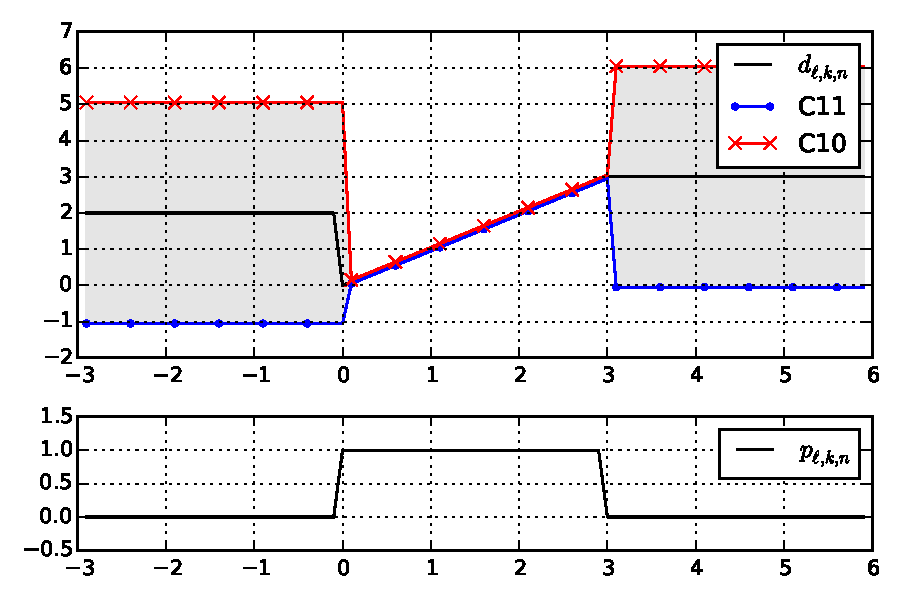
\includegraphics[width=0.45\textwidth,trim={0cm 0cm 0cm 0cm},clip]{phase_plot_fig_1.pdf}}
\subfigure[]{
\label{subfig:test1}
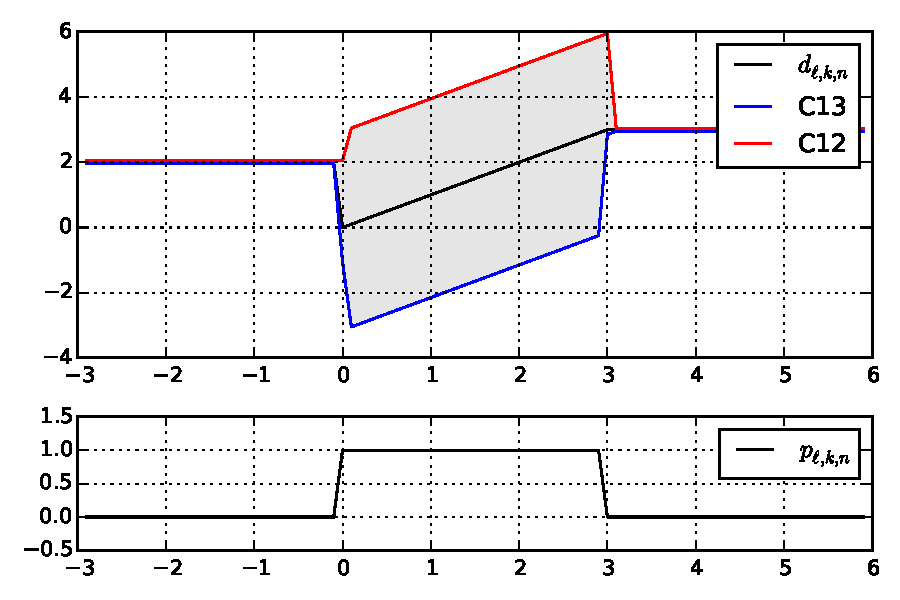
\includegraphics[width=0.45\textwidth,trim={0cm 0cm 0cm 0cm},clip]{phase_plot_fig_2.pdf}}
\subfigure[]{
\label{subfig:test1}
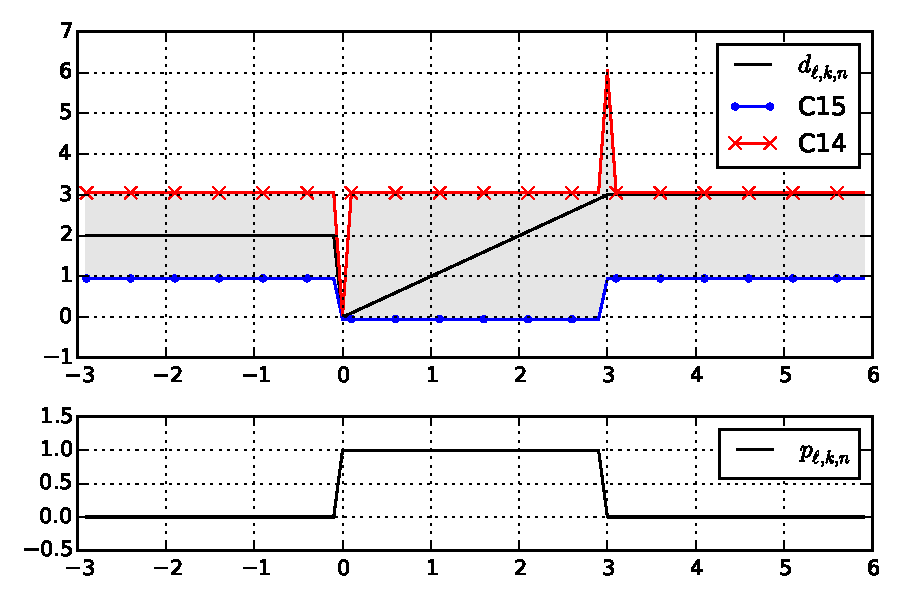
\includegraphics[width=0.45\textwidth,trim={0cm 0cm 0cm 0cm},clip]{phase_plot_fig_3.pdf}}
\subfigure[]{
\label{subfig:test1}
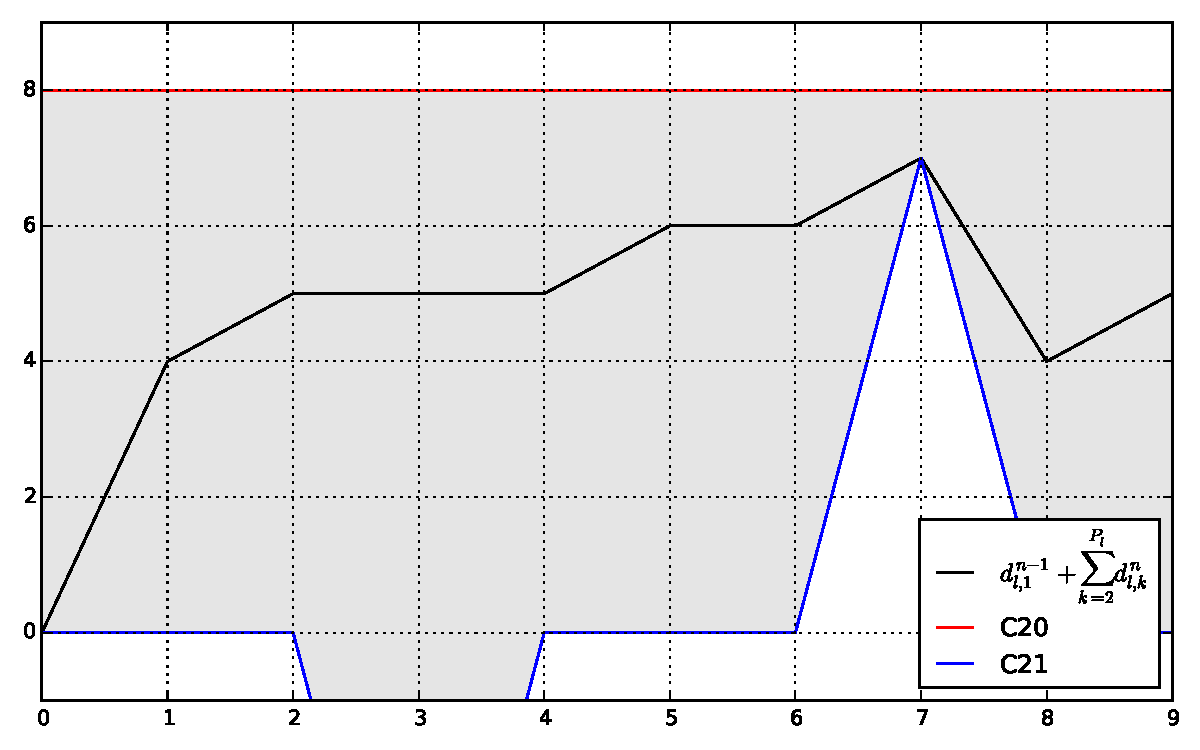
\includegraphics[width=0.45\textwidth,trim={0cm 0cm 0cm 0cm},clip]{phase_plot_fig_4.pdf}}
\caption{An example showing the phase and cycle time constraint envelopes. In (a), (b) and (c), $\PTMIN{\ell}{k}=1$ and $\PTMAX{\ell}{k}=3$, the duration of the previous activation was 2 and the duration of the current activation is 3. In (d), the total cycle time is 7 with $\CTMIN{\ell}=7$, $\CTMAX{\ell}=8$}
\label{fig:phase_plots}
\end{figure*}

\subsection{Objective Function}
Lin and Wang \cite{linwang} derive an objective function for the minimisation of total delay based on the difference between the cumulative departure and arrival curves at the origin and destination. However, such an approach requires the network to be cleared at the end of the optimisation period. We derive an objective function for the maximisation of flow in the network, and apply it to every queue in the network at $\qout{i}$,
\begin{equation}
maximise \left( \sum\limits_{n=1}^{\Nn} \sum\limits_{i=1}^{\Qn} (\TMAX - \tn + 1) \qout{i} + \sum\limits_{n=1}^{\Nn} \sum\limits_{i=1}^{\Qn} (\TMAX - \tn + 1) \inq{i} \right) 
\tag{O1}\label{eq:O1}
\end{equation}
And with the addition of the second $\inq[]{i}$ term, \ref{eq:O1} also ensures that \ref{eq:C1}, \ref{eq:C2}, and \ref{eq:C4} are also at their maximum upper bound.


\section{Analysis}

\subsection{Networks}
Three networks of increasing complexity were defined for performance analysis and comparison. The first consists of a two-way avenue with three traffic light controlled intersections with 3 one-way side streets, as shown in figure \ref{fig:network3}. The second is an extension of the first to include a second parallel two-way avenue and an additional 3 traffic lights to control the side streets, as shown in figure \ref{fig:network6}. And the third is a grid of three EW two-way avenues, with two NS two-way avenues and one NS one way street and a NE to SW diagonal one-way street, as shown in figure \ref{fig:network9}.
The traversal time of each queue in all three networks is set at 9 seconds (a distance of about 100m with a free flow speed of 50km/h). The maximum capacity of each queue is set at 60 cars. Flows are defined only straight ahead from the head of each queue into the tail of the next - there is no turning traffic, and in all cases the maximum flow rate is set at 5 cars per second. Each traffic light has two phases - NS and EW. The minimum phase time is 1 second and the maximum phase time is 3 seconds. The minimum cycle time of both the phases is 2 seconds and the maximum is 6.
For each network a background level of flow is first established and then later increased as a wave of higher volume traffic is injected into the network at some of the streets. Then all the traffic is allowed to clear the network before ending the simulation to support an analysis of the total travel time in the network. The details of the flow levels is given in tables \ref{tab:net1wave},  \ref{tab:net2wave} and  \ref{tab:net3wave}.

\subsection{Experiments}
With a CTM based model the $\DT[]$ must remain fixed through out the optimisation period, while the QTM supports non-homogeneous time steps mixed with homogeneous time steps. To exploit this we define a mutli-step solver that allows the time step of the plan to increase overtime. Such an increase will reduce the total number of variables for the same optimisation period compared to a homogeneous plan, with the trade off that the plan will be have less resolution over time. But this seems acceptable as the accuracy of the plan will also decrease overtime the further from the initial conditions.
We start by generating a plan for a longer horizon using an increasing time step so that the solver has greater visibility of the impact of an earlier planning decision across a larger part of the network for the same number of variables as a fixed time step. We then keep the first part of this plan where the accuracy is highest and discard the rest, where the time steps where larger. Once the retained section of plan has be carried out, we generate another long horizon plan and repeat (see figure \ref{fig:multiplan}.
We call the long term plan a major frame and the shorter section of a major frame that we retain, a minor frame. We use a minor frame of 10 seconds and increasing major frame sizes from 20 upwards and generate such mutlistep plans with both a homogeneous $\DT[]$ of 0.25 seconds and a non-homogenous $\DT[]$ ranging from fixed 0.25 second increments during the minor frame and the increasing linearly until 1 second at the horizon. We generated plans for all three networks using both the homogeneous $\DT[]$ major frames and the non-homogeneous $\DT[]$ major frames. For reference we also performed a full optimal solve using a fixed $\DT[]$ of 0.25 seconds. Once we have generated a set of minor frames, we combined them into a large fixed plan and simulate the flow of in the network with a fixed $\DT[]$ of 0.25, to support a fair comparison.

\begin{figure*}[t!]
\centering
%  trim={<left> <lower> <right> <upper>}
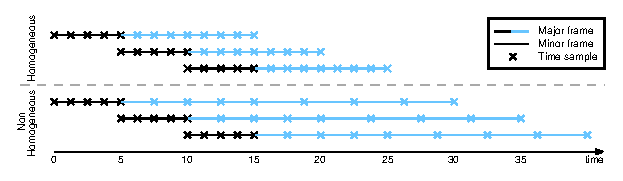
\includegraphics[width=1.0\textwidth]{non_homogeneous_control.eps}
\caption{Multi-step planning}
\label{fig:multiplan}
\end{figure*}


\begin{figure*}[t!]
\centering
%  trim={<left> <lower> <right> <upper>}
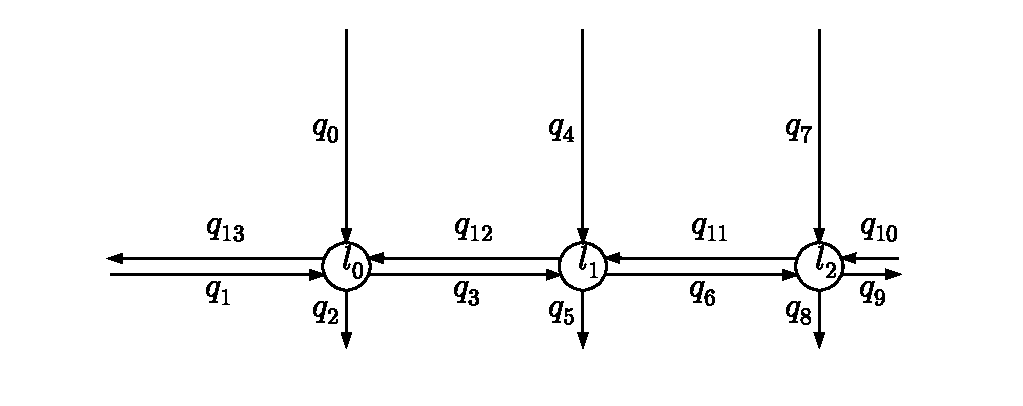
\includegraphics[width=0.75\textwidth]{network_3_lights}
\caption{Network 1}
\label{fig:network3}
\end{figure*}

\begin{table}[h]
\caption{Network 1 traffic parameters}
\label{tab:net1wave}
\centering
\begin{tabular}{cccccc}
\toprule
Queue & Background & End & Wave & Start &End\\ 
\midrule
$q_0$ & 1 & 85 & 1 & 55 & 70\\
$q_1$ & 2 & 85 & 4 & 55 & 70\\
$q_4$ & 4 & 85 & 4 & 55 & 70\\
$q_7$ & 4 & 85 & 4 & 55 & 70\\
$q_{10}$ & 2 & 85 & 4 & 55 & 70\\
\bottomrule\\
\end{tabular}
\end{table}


\begin{figure*}[t!]
\centering
%  trim={<left> <lower> <right> <upper>}
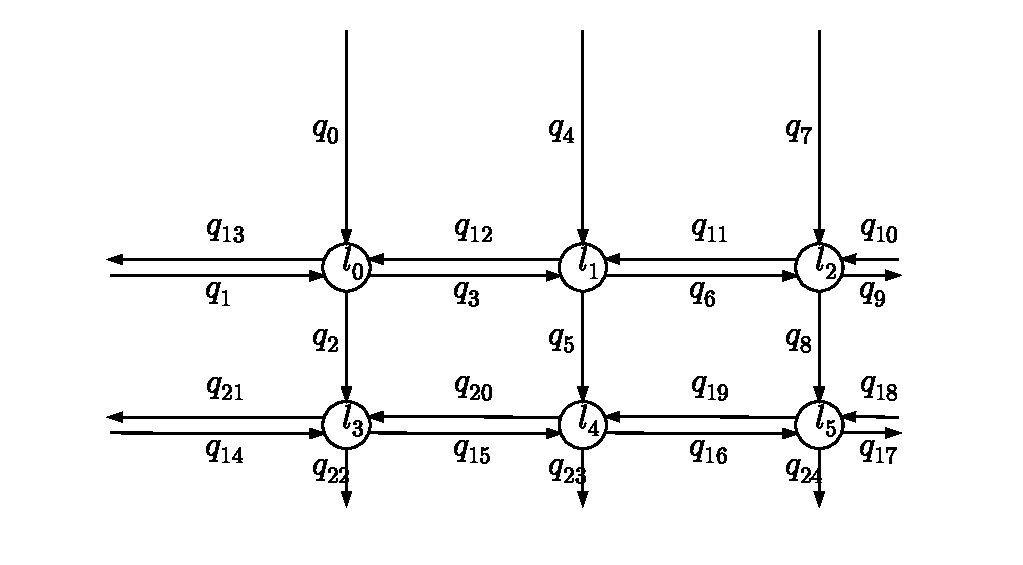
\includegraphics[width=0.75\textwidth]{network_6_lights}
\caption{Network 2}
\label{fig:network6}
\end{figure*}

\begin{table}[h]
\caption{Network 2 traffic parameters}
\label{tab:net2wave}
\centering
\begin{tabular}{cccccc}
\toprule
Queue & Background & End & Wave & Start &End\\ 
\midrule
$q_0$ & 1 & 85 & 1 & 55 & 70\\
$q_1$ & 2 & 85 & 4 & 55 & 70\\
$q_4$ & 4 & 85 & 4 & 55 & 70\\
$q_7$ & 4 & 85 & 4 & 55 & 70\\
$q_{10}$ & 2 & 85 & 4 & 55 & 70\\
$q_{14}$ & 4 & 85 & 4 & 55 & 70\\
$q_{18}$ & 2 & 85 & 4 & 55 & 70\\
\bottomrule\\
\end{tabular}
\end{table}


\begin{figure*}[t!]
\centering
%  trim={<left> <lower> <right> <upper>}
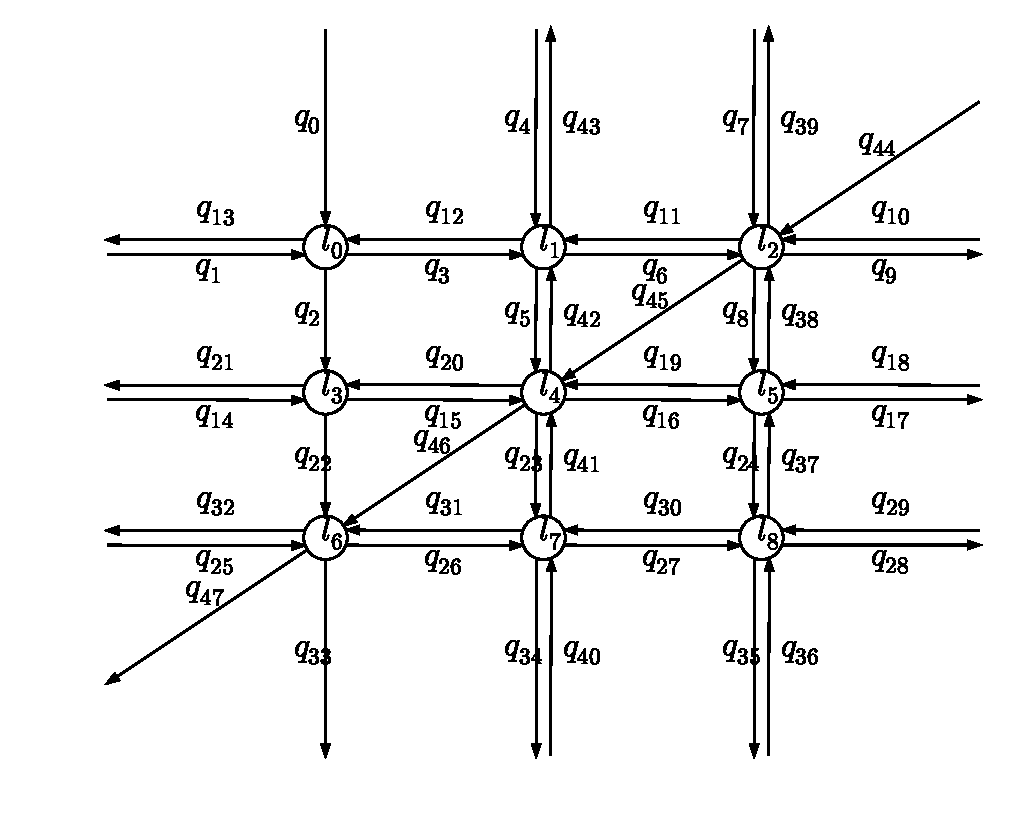
\includegraphics[width=0.75\textwidth]{network_9_lights}
\caption{Network 3}
\label{fig:network9}
\end{figure*}


\begin{table}[h]
\caption{Network 3 traffic parameters}
\label{tab:net3wave}
\centering
\begin{tabular}{cccccc}
\toprule
Queue & Background & End & Wave & Start &End\\ 
\midrule
$q_0$ & 1 & 85 & 1 & 55 & 70\\
$q_1$ & 2 & 85 & 4 & 55 & 70\\
$q_4$ & 4 & 85 & 4 & 55 & 70\\
$q_7$ & 4 & 85 & 4 & 55 & 70\\
$q_{10}$ & 2 & 85 & 4 & 55 & 70\\
$q_{14}$ & 4 & 85 & 4 & 55 & 70\\
$q_{18}$ & 2 & 85 & 4 & 55 & 70\\
$q_{25}$ & 4 & 85 & 4 & 55 & 70\\
$q_{29}$ & 2 & 85 & 4 & 55 & 70\\
$q_{36}$ & 2 & 85 & 4 & 55 & 70\\
$q_{40}$ & 2 & 85 & 4 & 55 & 70\\
$q_{44}$ & 2 & 85 & 4 & 55 & 70\\
\bottomrule\\
\end{tabular}
\end{table}

\section{Results}

We compared the performance of non-homogeneous and homogeneous $\DT[]$ in two ways: comparing the decrease in total travel time with increasing major frame size. And analysing the distribution of delay in each queue of the network. Figure \ref{fig:results} (a), (c) and (e) show a comparison between the number of time samples used in the major frame vs the \% improvement in total travel time. It can be seen that using a non homogenous $\DT[]$ converges towards the optimum more quickly than the homogeneous $\DT[]$ for the same number of time samples. Figure \ref{fig:results} (b), (d) and (f) show a comparison of distribution of delay across the network. This gives us an indication of the quality of the solution in terms of the number of vehicles that experience significant delay and if the plan may be starving some parts of the network.  The plots show three comparisons: at the point where the non-homogeneous $\DT[]$ first converges on the optimum solution, where the homogeneous $\DT[]$ first converges on the optimum solution, and the optimum solution. With all three networks the quality of the solutions improves or stays the same using an non-homogeneous $\DT[]$ compared to a homogeneous $\DT[]$.
Finally, figure \ref{fig:cumu} shows the how cumulative arrival and departure curves and the delay develop over time for $q_1$ of network 2. Figure \ref{fig:cumu} (a) shows the comparison at the point where the non-homogeneous $\DT[]$ first converges and shows that with the longer major frame of the non-homogeneous $\DT[]$, it is able to adopt a better signal plan early on to anticipate the wave of traffic that arrives at about the 55 second point, while the homogeneous $\DT[]$ with its shorter major frame initially prioritises the side street ($q_0$, $q_2$, $q_{22}$) over $q_1$ resulting in significant delay once the wave of traffic arrives. Once homogeneous $\DT[]$ has converged in Figure \ref{fig:cumu} (b), both plans are close to the optimum shown in Figure \ref{fig:cumu} (c).

\begin{figure*}[t!]
\centering

%  trim={<left> <lower> <right> <upper>}
\subfigure[]{
\label{subfig:travel_time_3}
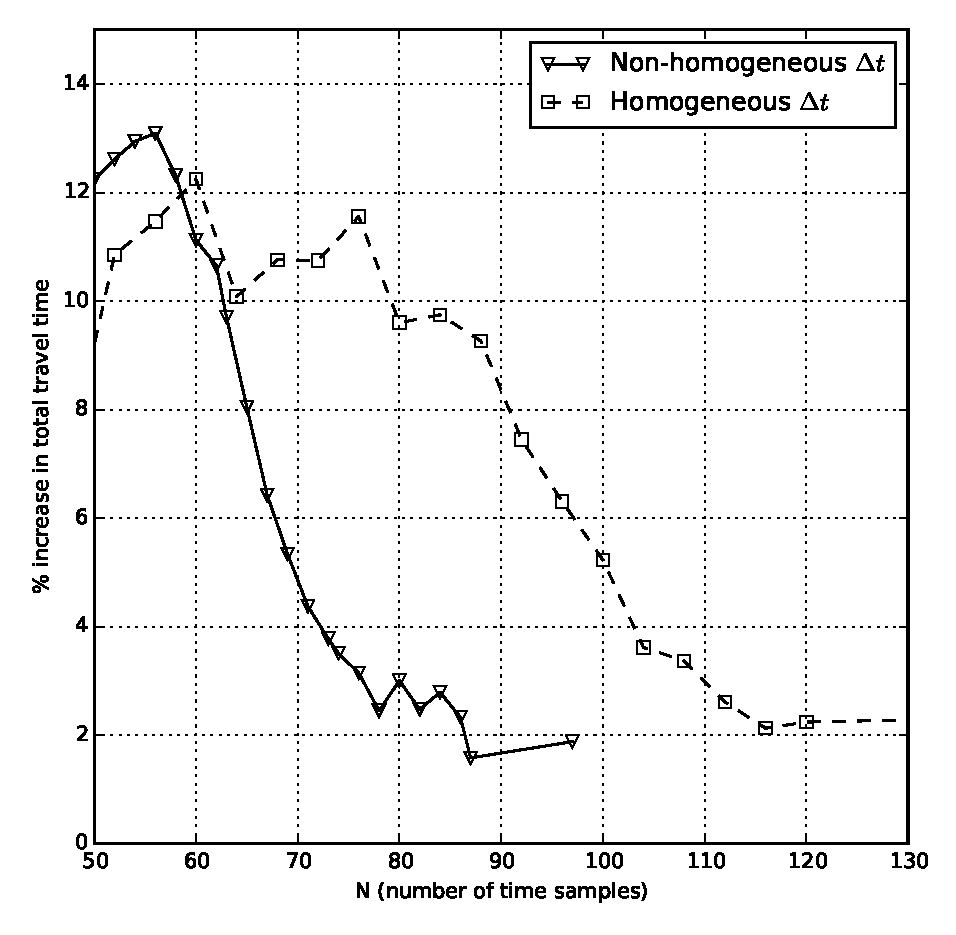
\includegraphics[width=0.4\textwidth]{samples_plot_3_lights}}
\subfigure[]{
\label{subfig:delay_3}
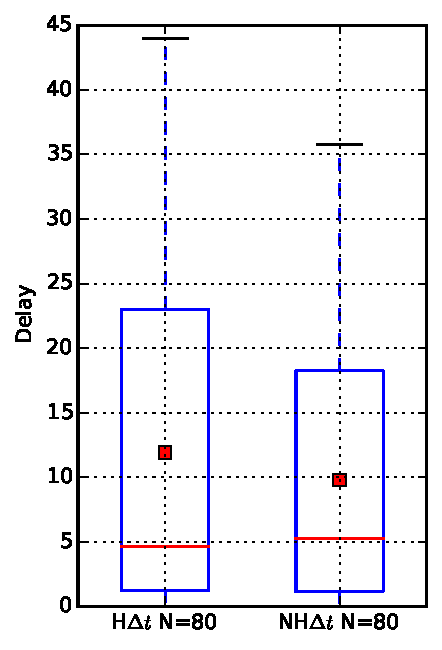
\includegraphics[keepaspectratio,height=0.3\textwidth]{box_plot_early_3l.pdf}
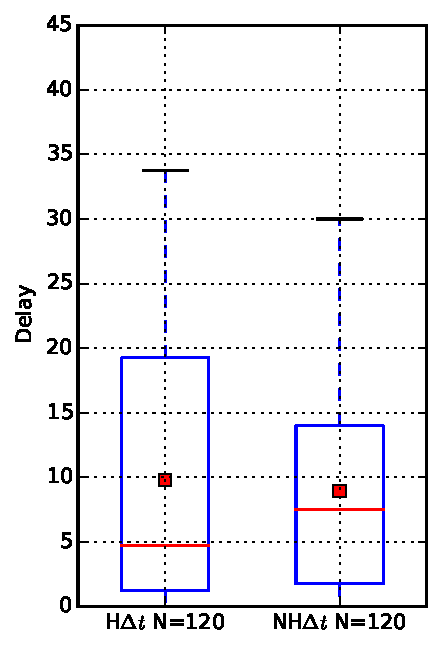
\includegraphics[keepaspectratio,height=0.3\textwidth]{box_plot_converg_3l.pdf}
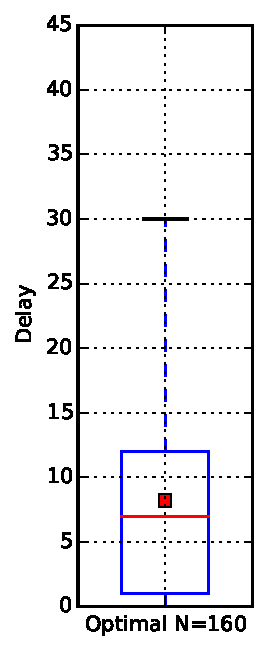
\includegraphics[keepaspectratio,height=0.3\textwidth]{box_plot_final_3l.pdf}}

\subfigure[]{
\label{subfig:travel_time_6}
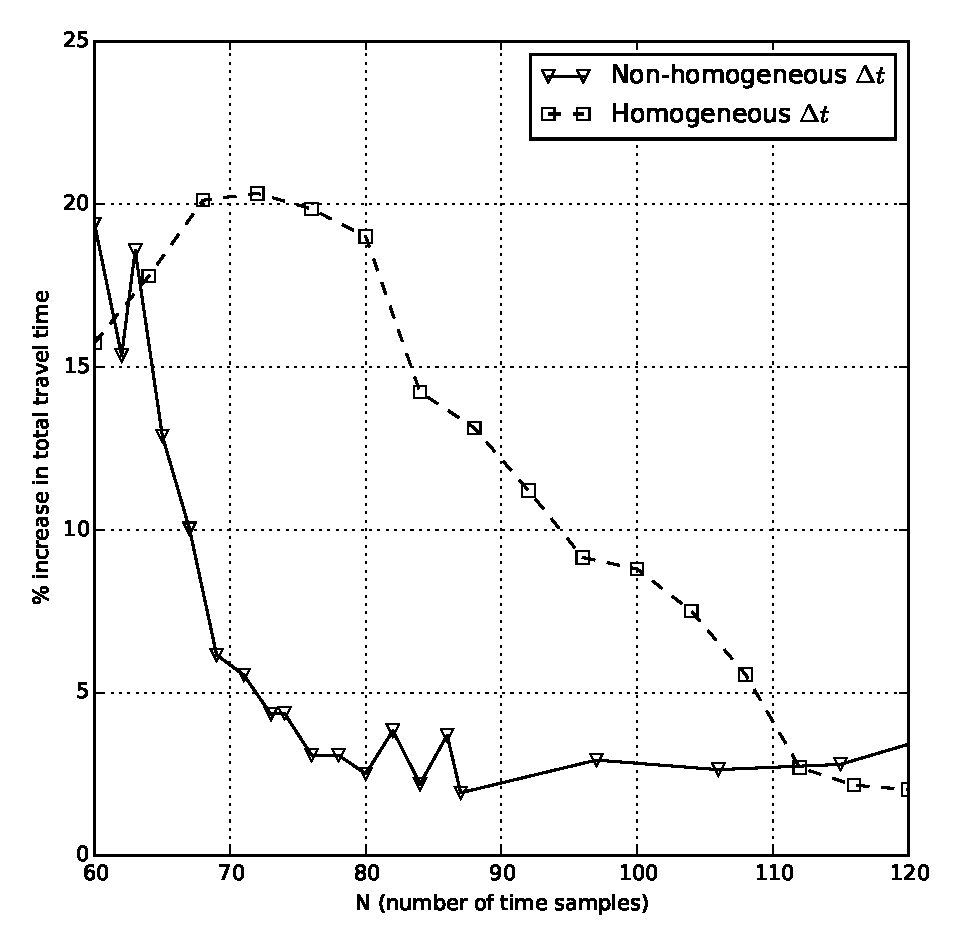
\includegraphics[width=0.4\textwidth]{samples_plot_6_lights}}
\subfigure[]{
\label{subfig:delay_6}
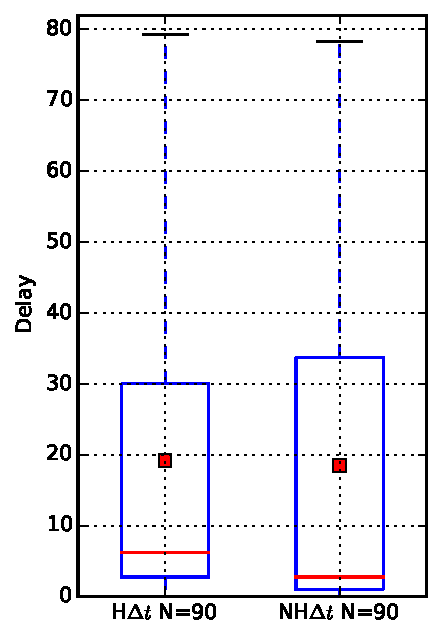
\includegraphics[keepaspectratio,height=0.3\textwidth]{box_plot_early_6l.pdf}
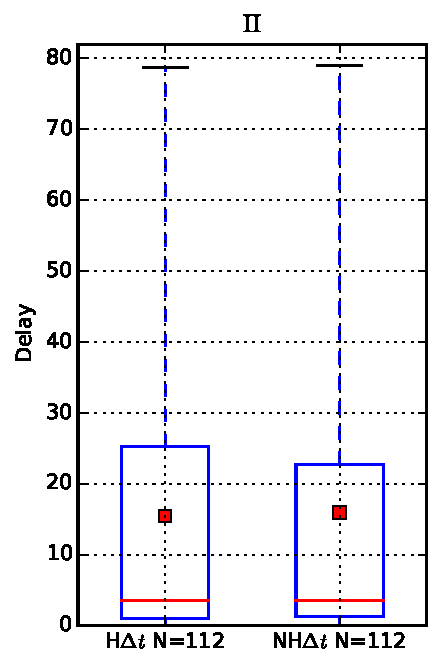
\includegraphics[keepaspectratio,height=0.3\textwidth]{box_plot_converg_6l.pdf}
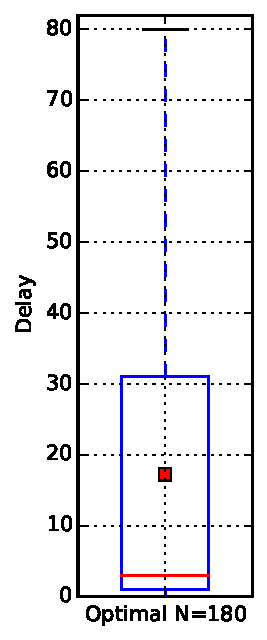
\includegraphics[keepaspectratio,height=0.3\textwidth]{box_plot_final_6l.pdf}}

\subfigure[]{
\label{subfig:travel_time_9}
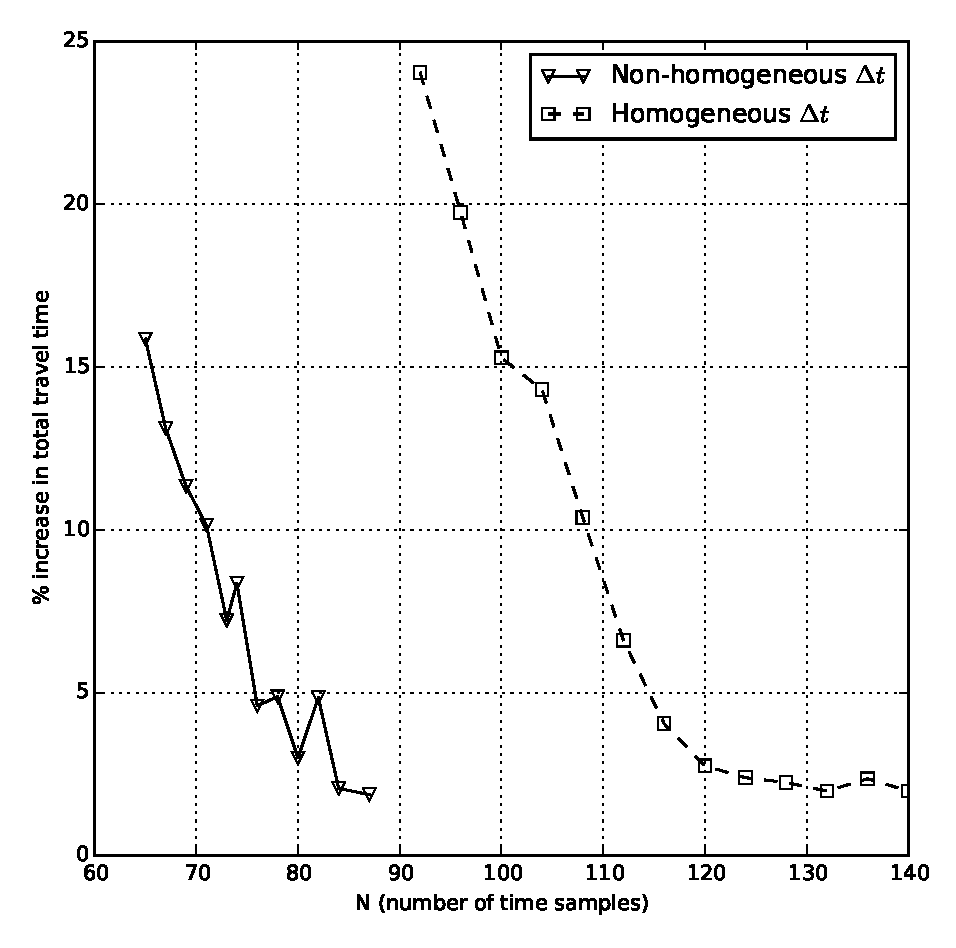
\includegraphics[width=0.4\textwidth]{samples_plot_9_lights}}
\subfigure[]{
\label{subfig:delay_9}
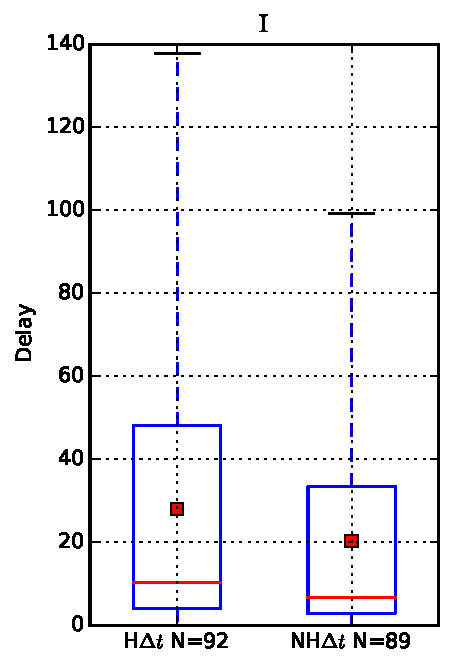
\includegraphics[keepaspectratio,height=0.3\textwidth]{box_plot_early_9l.pdf}
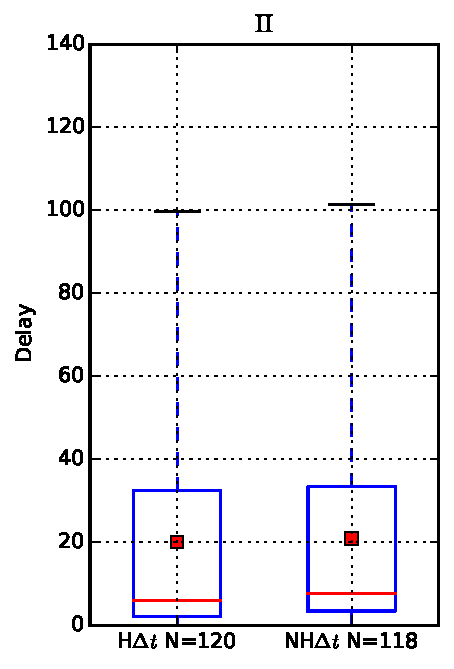
\includegraphics[keepaspectratio,height=0.3\textwidth]{box_plot_converg_9l.pdf}
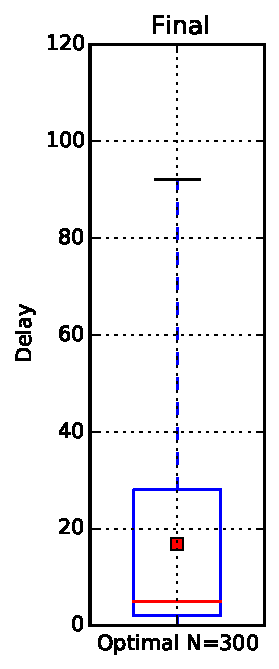
\includegraphics[keepaspectratio,height=0.3\textwidth]{box_plot_final_9l.pdf}}
\caption{Results for the three networks showing the comparitive \% improvement in total travel time for the network between using a homogeneous $\DT[]$ and a non-homogeneous $\DT[]$, and the distribution of delay time at the convergence point of non-homogeneous $\DT[]$, the convergence point of homogeneous $\DT[]$ and for the fully solved optimal solution. (a) and (b) 3 light avenue, (c) and (d) 6 light grid, and (e) and (f) 9 light grid,}
\label{fig:results}
\end{figure*}

\begin{figure*}[t!]
\centering

%  trim={<left> <lower> <right> <upper>}
\subfigure[]{
\label{subfig:cumu1}
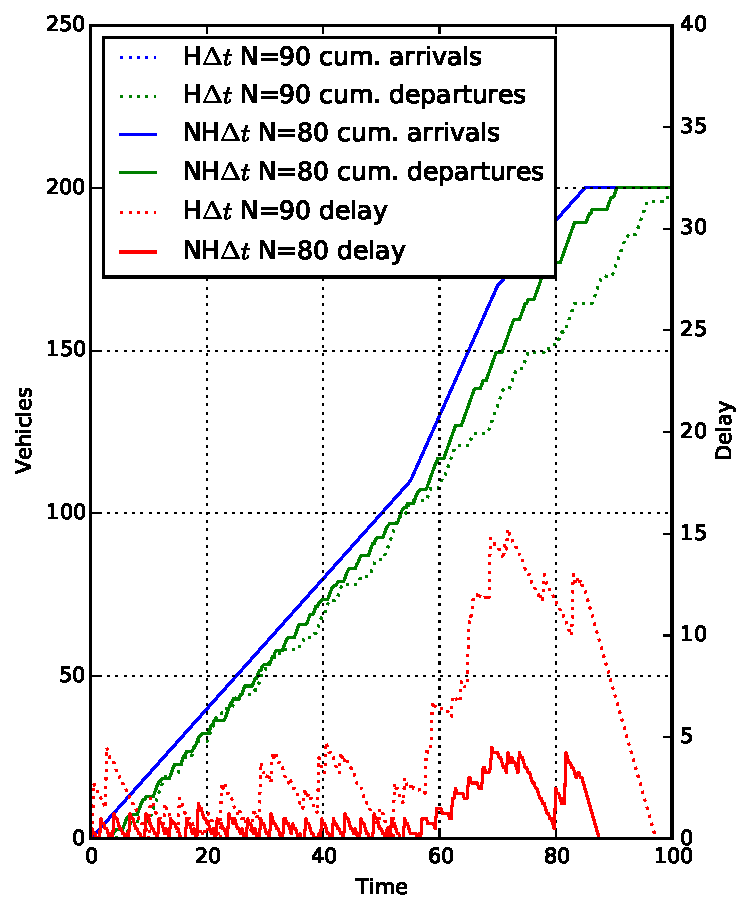
\includegraphics[width=0.32\textwidth]{cum_plot_early_6l.pdf}}
\subfigure[]{
\label{subfig:cumu2}
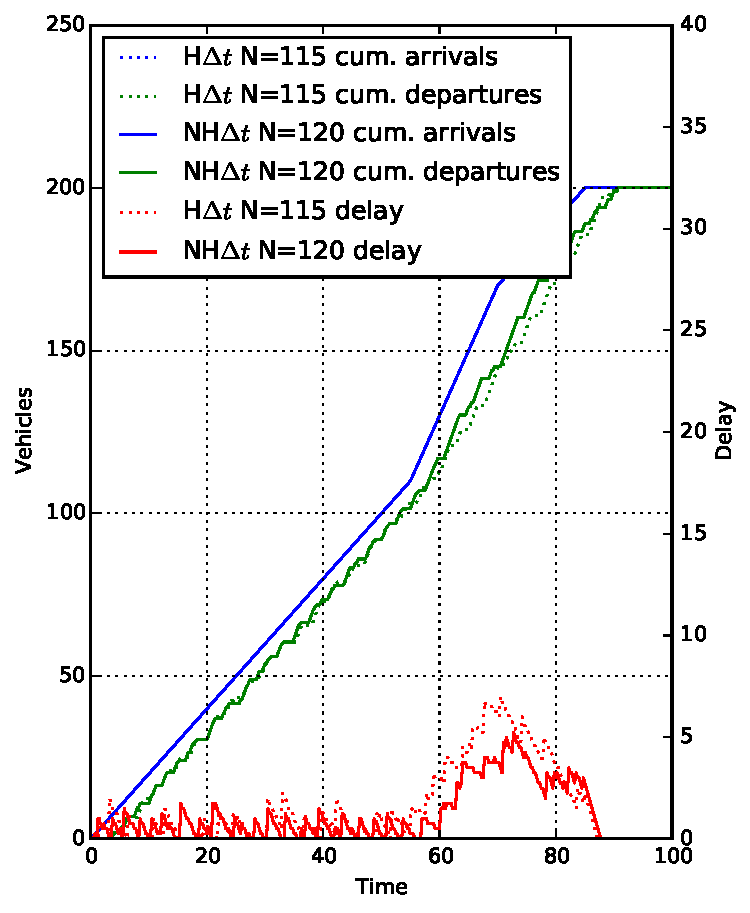
\includegraphics[width=0.32\textwidth]{cum_plot_converg_6l.pdf}}
\subfigure[]{
\label{subfig:cumu3}
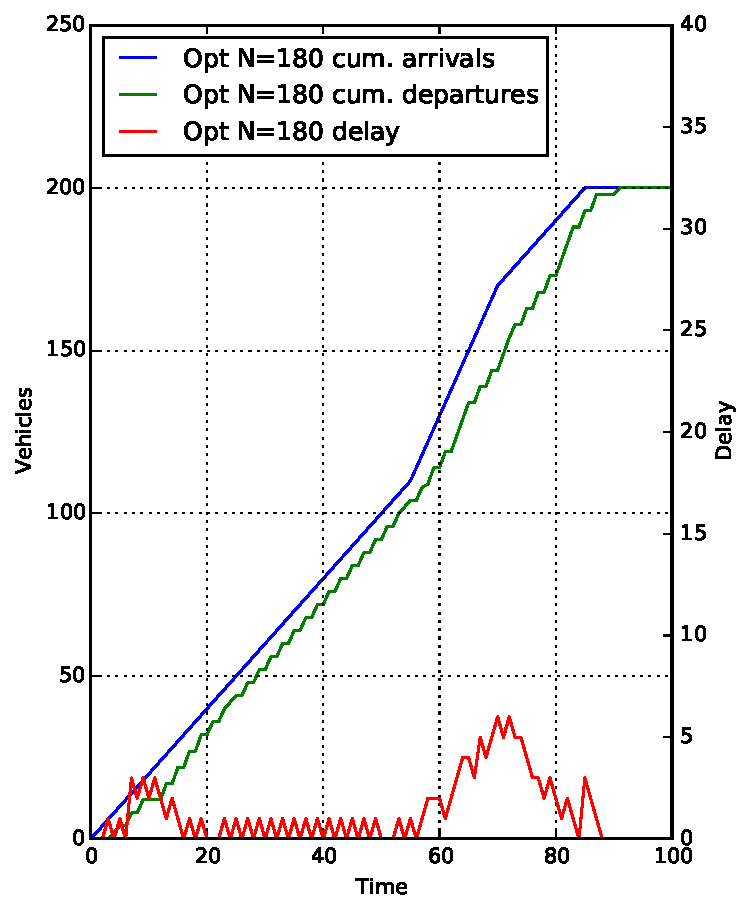
\includegraphics[width=0.32\textwidth]{cum_plot_final_6l.pdf}}
%\includegraphics[width=0.25\textwidth,trim={3cm 1.5cm 3cm 2.3cm},clip]{Satellite_Augmentation/test_17.eps}}
\caption{Cumulative arrival and departure curves and delay for queue 1 in the 6 light grid. (a) at the convergence point of the non-homogeneous $\DT[]$ it is near to the optimum solution while homogeneous $\DT[]$ lags behind (b) at the convergence point of homogeneous $\DT[]$ both are near optimum, and (c) the fully solved optimal solution}
\label{fig:cumu}
\end{figure*}

\section{Conclusion}
We have demonstrated that by exploiting the non-homogeneous time steps supported by the QTM, we are able to scale the model up to larger networks and using the same number of binary variables as a homogeneous time step, and with the same quality of a homogeneous solution using more binary variables.

\bibliographystyle{trb}
%\bibliography{TRBLaTeX}
\begin{thebibliography}{10}

\bibitem{linwang}
W.~Lin and C.~Wang, \emph{An Enhanced 0-1 Mixed-Integer LP Formulation for Traffic Signal Control}, IEEE Transactions on Intelligent Transport Systems, Vol. 5, No. 4, pp. 238--245, December 2004.
\bibitem{daganzo}
C. F. Daganzo, \emph{The cell transmission model: A dynamic representation of highway traffic consistent with the hydrodynamic theory}, Transport. Res. B., vol. 28, no. 4, pp. 269�287, 1994.
\end{thebibliography}

% End line numbering
\nolinenumbers
\end{document}
